\cotefile{157-1}
\scanpage{166}
\mspage{24}

Nous nous plaçons \inserted{\unsure{donc}} dans l'hypothèse où PS1 est satisfait (puisque b), c') et d) impliquent PS1), donc où \inserted{on est sous} les conditions équivalentes de 2.5. -- $\unsure{\mathscr X|\mathcal X}$ est loc. irréductible. Considérons \inserted{alors} la condition PS2, et prouvons qu'elle est impliquée tant par b), que par c'), et qu'elle implique \unsure{c'|a'}. Elle signifie que pour une double-flèche $a\overset{u}{\underset{v}{\unsure{=|\rightrightarrows}}}b$ dans $S$, \unsure{le|leur} \deleted{produit fibré} \inserted{\unsure{conoyau|noyau}} dans $S^\wedge$, ou ce qui revient au $=$ dans $\mathscr X^\wedge=S^\sim\subset S^\wedge$, est ``non vide''. On peut l'écrire sous la forme d'un produit fibré

\diagram{\begin{tikzcd}[ampersand replacement=\&]
a \arrow[r,"{(u,v)}"] \& b\times b \\
{\operatorname{Ker}(u,v)} \arrow[u] \arrow[r] \& b \arrow[u,"{\unsure{\mathrm{diag}|\mathrm{di}\,\Theta}}"']
\end{tikzcd}}

Ici par hyp. $a$ et $b$ sont des objets $0$-connexes de $\mathscr X^\wedge$ (comme ds $S$ l'étaient), \inserted{c) est vérifié ($\mathscr X$ loc. irréd. et ses \unsure{composantes} ttes $0$-connexes)} \deleted{Si $b\times b$ est $0$-connexe, alors si} donc $b\times b$ est \unsure{aussi} $0$-connexe, comme produit de deux objets \inserted{$0$-connexes} \unsure{sur une} \uline{$=$ \unsure{composante} connexe} ce qu'elle est \deleted{\unsure{est}} $0$-connexe\unsure{;} Comme $\mathscr X\times\mathscr X$ est loc. irréductible, il s'ensuit que le produit fibré est \deleted{\unsure{non}} vide (2.8.), donc $\mathrm{b)}\Longrightarrow\mathrm{d)}$. Prouvons $\unsure{\mathrm{d)}|\mathrm{c')}}\Longrightarrow\unsure{\mathrm{a)}|\mathrm{d)}}$ \unsure{i.e. si} \deleted{\unsure{les produits|que les produits} fibrés $a\times_{\unsure{\mathscr X|x}}b$ \unsure{($a,b$ ds $S$)} sont $0$-connexes, donc PS2 est satisfait,}

% archive sheet number: 166
\scanpage{167}
\mspage{25}

$S$ est \deleted{\unsure{filtrant|f}} loc. cofiltrante, donc \deleted{le topos $\unsure{\mathscr X|\mathcal X}$ est \unsure{d.}} les topos induits $\mathscr X_{/W}$, où $W$ est $0$-connexe, sont tot. $0$-connexes. Ce topos induit est décrit par le site $S_{/W}$, i.e $S_{/W}$ est un syst. de générateurs. Or si $S$ est loc. \deleted{\unsure{préfilt.|pfilt.}}cofiltrant, $S_{/W}$ (étale sur $S$) l'est aussi. Donc \deleted{il reste à prouver} OPS $W=e$, et à prouver que si $S$ est \inserted{loc.} \deleted{\unsure{pro.}}cofiltrante et $\mathscr X$ $0$-connexe, donc $\mathscr X$ est tot. $0$-connexe. \deleted{\unsure{D'après}} \inserted{Ajoutons} \deleted{2.3. il suffit de prouver}  que $\mathscr X$ $0$-connexe \deleted{\unsure{si et que}}\inserted{équivaut à} $S$ $0$-connexe -- il faudrait quand $=$ l'expliciter :

\uline{Lemme} 2.9. \deleted{\unsure{\(\mathscr X\)}} Soit $\mathscr X$ un topos, $S\subset\mathscr X^\wedge$ une \deleted{\unsure{système de}} \inserted{sous-catégorie pleine} génératrice formée d'objets \uline{$0$-connexes}. \reversemarginpar\margin{\rule{0.4pt}{13ex}}\normalmarginpar Alors $\mathscr X$ est $0$-connexe ssi $S$ l'est -- plus \deleted{\unsure{précisément}} \inserted{généralement}, l'ensemble \inserted{ordonné} des sous-objets à la fois ouverts et fermés de $S$ dans Cat, \deleted{\unsure{i.e. des}} ou encore des \deleted{cribles} \deleted{qui sont des \unsure{co}} sous-objets ouverts $=$ cribles de $S$ qui sont aussi fermés i.e des cocribles) est \deleted{\unsure{Donn.}} \deleted{\unsure{correspondance}}, celui des \deleted{sous-objets} \deleted{à la fois \unsure{ouv.}} \unsure{sommandes|sous-ensembles} \unsure{directs|discrets} de $\mathscr X$.

Je l'ai utilisé tacitement dans la démonstration de 2.8, pour le topos induit $\mathscr X_{/W}$. Je n'explicite pas la démonstration.

Ainsi, \unsure{revenant à|concernant} la dém. de $\mathrm{d)}\Rightarrow\mathrm{a)}$ de 2.6, \deleted{\unsure{S}} \unsure{$S$ étant|étant} $0$-connexe et loc cofiltr\unsure{ant|é},

% archive sheet number: 167
\scanpage{168}
\mspage{26}

est en fait cofiltrante\deleted{\unsure{, donc}}, \unsure{Donc|donc} pour deux objets $a,b$ de $S$, $\exists\ c$ avec $c\longrightarrow a$, $c\unsure{\mathbin{-}|\longrightarrow}b$ (condition PS1$'$, plus forte que PS1). Pour prouver que $\unsure{\mathscr X|\mathcal X}$ est tot. $0$-connexe, on est réduit à prouver \inserted{par 2.3.} que les $a\times b$ dans $\mathscr X^\wedge$ sont $0$-connexes. Par 2.9, il revient au $=$ de prouver qu'ils sont $0$-connexes dans $S^\wedge$. Donc on est ramené à prouver le

\uline{Lemme 2.10}. Soit $S$ une catégorie cofiltrante. Si $a,b$ sont deux objets de $S$, $a\times b$ est un objet $0$-connexe de $S^\wedge$.

On voit de suite qu'il \deleted{\unsure{revient au même de}} \inserted{suffit de prouver (et} en fait il revient au $=$, compte tenu que $a\times b$ est loc. \deleted{\unsure{donc}} \inserted{irréductible)} que si on a deux flèches

% slanted
\margin{\deleted{\uline{\unsure{Lemme}} Soit $f$ \unsure{un|une} \illegible{1}. Alors $f$ \illegible{2} \unsure{est propre à}}}

\diagram{\begin{tikzcd}[ampersand replacement=\&]
x \arrow[r] \& a\times b \\
\& y \arrow[u]
\end{tikzcd}}

alors $x\times_{a\times b}y\ne\varnothing$ i.e $\exists\,z$ dans $S$ rendant commutatif

\diagram{\begin{tikzcd}[ampersand replacement=\&]
x \arrow[r] \& a\times b \\
z \arrow[u] \arrow[r] \& y \arrow[u]
\end{tikzcd}}

Or par PS1$'$ il existe bien un $z$ s'envoyant dans $x$ et dans $y$, mais les deux flèches composées

\[
z\rightrightarrows a\times b
\]

i.e. donnant des doubles flèches

\[
z\rightrightarrows a \tag*{$(*)$}
\]

\[
z\rightrightarrows b, \tag*{$(*')$}
\]

peuvent n'être pas égales. Mais par PS2,

% archive sheet number: 168
\scanpage{169}
\mspage{27}

on peut trouver

\[
z'\overset{\displaystyle\longrightarrow}{\deleted{\unsure{\longleftarrow|\longrightarrow}}}z
\]

égalisant la double-flèche $(*)$, donc \deleted{\unsure{OPS}} que celle-ci est déjà triviale. Appliquant encore une fois PS2, \deleted{\unsure{on trouve}} \inserted{par} un $z''\unsure{\mathbin{-}|\longrightarrow}z'$, on égalise de $=$ \unsure{la|le} double flèche $(*')$, et on gagne. On a donc prouvé, finalement

\diagram{\begin{tikzcd}[ampersand replacement=\&]
a \arrow[r,Leftrightarrow] \arrow[d,Rightarrow] \& a' \arrow[r,Rightarrow] \& b \arrow[r,Leftrightarrow] \& d\,(=\mathrm{PS1}+\mathrm{PS2})\\
c \arrow[r,Leftrightarrow] \& c' \& \&
\end{tikzcd}}

Mais pas l'implication inverse. En d'autres termes, si les topos induits $\unsure{\mathscr X|\mathcal X}_{/a}$, pour $a$ de $S$, sont \deleted{\unsure{on a expliqué}} tot. $0$-connexes, je \deleted{\unsure{ne}} n'ai pas prouvé qu'il en est de $=$ des $\mathscr X_{/W}$, $W$ un objet $0$-conn. \uline{quelc.} de $\mathscr X^\wedge$. \deleted{Notons que c) signifie \unsure{ici} que les produits fibrés de\unsure{ux}} \inserted{Ainsi, on \deleted{\unsure{est}} en est au point suivant}

\uline{\unsure{Proposition|Prop. Corollaire}} 2.11. Soit $X$ dans Cat. \deleted{Soit} Si $X$ est \inserted{loc} filtrante \inserted{\unsure{à g.|i.e.}}, alors \deleted{$X$ est $0$-connexe$,$} les produits fibrés $a\times_{\unsure{X|x}}b$ d'objets de $X$ sont des objets $0$-connexes de $X^\wedge$, \deleted{\unsure{ce qui}} \inserted{et cette} condition à son tour implique PS1, i.e. que $X$ est loc. irréductible. Mais en \unsure{partant|présence} de cette hypothèse PS1, ou $X$ loc irréductible, la condition sur les produits fibrés $a\times_{\unsure{x|\vphantom{x}}}b$ équivaut à \unsure{la|le} \unsure{suivante|suivant} : \deleted{pour tout \unsure{diagramme}} pour tout diagramme traits pleins

% archive sheet number: 169
\scanpage{170}
\mspage{28}
\diagram{\begin{tikzcd}[ampersand replacement=\&]
c \arrow[r] \& a\times_{\unsure{x|a}}b\\
e \arrow[u,dashed] \arrow[r,dashed] \& d \arrow[u]
\end{tikzcd}}

, avec $x,a,b,x,c,d$ dans $\unsure{X|A}$, on peut compléter en un diagramme \uline{commutatif}, avec $e$ dans $X$. En d'autres termes, tout diagramme commutatif à traits pleins ci-dessous se complète en y ajoutant un ``objet initial'' $e$

% margin note written sideways
\reversemarginpar\margin{$\times$ Elle signifie que $X$ satisfait PS1, et \deleted{\unsure{que p.}} la condition \uline{PS$'2$} \deleted{\unsure{Pour}} Tout diagramme comm. \diagram{\begin{tikzcd}[ampersand replacement=\&,column sep=small] a\arrow[r,shift left=.5ex]\arrow[r,shift right=.5ex]\&b\arrow[r]\&x\end{tikzcd}} s'insère dans un diagr. comm. \diagram{\begin{tikzcd}[ampersand replacement=\&,column sep=tiny] y\arrow[r]\&a\arrow[r,shift left=.5ex]\arrow[r,shift right=.5ex]\&b\arrow[r]\&x\end{tikzcd}}}\normalmarginpar

\diagram{\begin{tikzcd}[ampersand replacement=\&]
\& c\arrow[r]\arrow[ddr]\arrow[rrd,"{\deleted{\unsure{\longrightarrow}}}" description,rightsquigarrow] \& a\arrow[dr] \& \\
e\arrow[ur,dotted]\arrow[dr,dotted] \& \& \& x\\
\& d\arrow[uur]\arrow[r] \& b\arrow[ur] \&
\end{tikzcd}}

\margin{il suffit d'exiger pour $e$ la commutativité des deux carrés $(e c b d)$ et $(e d a c)$}

Cette condition est donc impliquée par $X$ \inserted{loc.} cofiltrant, et elle est satisfaite aussi \inserted{(par ce qui précède)} \inserted{plus généralement} \unsure{ssi|si} les $X_{/x}$ sont cofiltrants.$^{\times}$ Mais la \unsure{réciproque|réciprocité} est-elle vraie -- cette condition de \unsure{totale} $0$-connexité des $X_{/a}$ implique-t-elle que $X$ \inserted{soit tot. $0$-connexe ?} \deleted{Mais} Je n'ai pas d'exemples où les $X_{/x}$ sont \inserted{ou seulement même des $X$ $0$-connexes, les $X_{/x}$ cofiltr., sans que $X$ \unsure{même} soit cofiltr.} sans que $X$ soit loc. cofiltrant ;

% slanted
\reversemarginpar\margin{si et seulement si ?}\normalmarginpar

% slanted
\reversemarginpar\margin{Mais il y a un \unsure{de|des} \uuline{contre-exple} évident, si $X$ est un \uline{groupoïde}, \unsure{or|on} \unsure{tous} les $X_{/x}$ sont $\simeq e$ donc cofiltrants, mais $X$ lui n'est \deleted{loc.} cofiltrant (\unsure{i.e.} \unsure{contractile}) que si $X$ est \unsure{équivalent|discret} \unsure{à $e$}. \unsure{$\pi_1\ne1$}. \unsure{Voir} ci. \unsure{Si ça est vrai|Si c'est vrai}, \unsure{on tient donc} \unsure{2.8 bis} \unsure{un} \unsure{tel} que les $X_{/x}$ sont cofiltrants, \unsure{Ctr ex. ?} mais $X$ \unsure{a un $\pi_1$|ne l'est} \unsure{non|pas} \unsure{trivial|cofiltrant}.}\normalmarginpar

\unsure{ou} d'exemples où les \deleted{\unsure{produit}} $X_{/x}$ sont $0$-connexes, \deleted{\unsure{tels}} que les $\unsure{X'_{/x}|X_{/x}}$ soient cofiltrants. Mais notons le

\uline{Corollaire} 2.12 : Les conditions équivalentes de \deleted{\unsure{2,}} a) a') b) d) [$\,$à l'exclusion de c, c', plus faibles apparemment$\,$] du th. 2.6.

% archive sheet number: 170
\scanpage{171}
\mspage{29}
% slanted
\reversemarginpar\margin{NB $\unsure{\mathscr X|\mathcal X}_{/x}$ inutile}\normalmarginpar

équivalent \deleted{\unsure{encore}} à la suivante e) $\forall\,a$ dans $S$, le \deleted{\unsure{caté}} topos induit $\mathscr X_{/x}$ \deleted{\unsure{est $0$-connexe} et \unsure{irréductible}, \unsure{totalement connexe}} et le topos induit \deleted{\unsure{sur}} $\mathscr X_{/x\times x}$ est \inserted{irréductible.} \deleted{\unsure{e)}} ou encore à la suivante. e') $\forall\,x$ dans $S$, $(S^\wedge_{/x})$ \deleted{\unsure{est irréductible,}} et $S^\wedge_{/x\times x}$ \deleted{est tot. $0$-connexe} sont irréductibles, i.e. $S_{/x}$ et \inserted{$S_{/x\times x}$ sont irréductibles.} \deleted{\unsure{cofiltrants}}

% slanted
\reversemarginpar\margin{$S_{/x}$ inutile, car $\overset{\mathrm{diag}}{x\longrightarrow x\times x}$ est une \unsure{imm.|immersion} ouverte \unsure{non vide}, donc si $x\times x$ est irréd, $x$ l'est aussi. Mais il revient \unsure{donc} au $=$ de dire que les $S_{/x}$ sont irréductibles (condition PS$^{\unsure{x|1}}$1, cf. 2.8, p.~21) \uline{et} que les $x\xrightarrow{\mathrm{diag}}x\times x$ sont dominantes (ce qui implique en effet que $x\times x$ est irréd.) et ceci redonne immédiatement la forme PS$^{x}$2 de la condition cofiltrante.}\normalmarginpar

C'est la forme ``topologique'' la plus faible en apparence que je peux trouver pour la condition $S$ loc cofiltrante, i.e. $\mathscr X$ (\unsure{ou} \deleted{\unsure{Top}} Top$(S)$, ou \unsure{disons|discr.}) \deleted{à la fois loc irréduc et} loc tot. \deleted{\unsure{asph.}} $0$-connexe.

\uline{Définition} 2.13. On dit qu'un topos $\mathscr X$ est \uline{\unsure{localmt|localement}} tot \uline{$0$-connexe} s'il satisfait aux conditions équivalentes a,a',b,d du th. 2.6, i.e. si $\mathscr X$ est loc connexe et si \inserted{de plus} \deleted{\unsure{tout}} topos induit $0$-connexe est tot. $0$-connexe -- \unsure{i.e.} \unsure{encore} le produit fibré de deux objets $0$-connexes sur un troisième est $0$-connexe. Il revient au $=$ de dire que \deleted{\unsure{tz}} \inserted{lorsque \uline{une}} sous catégorie pleine génératrice $S$ de $\mathscr X^\wedge$, formée d'objets $0$-connexes est loc. cofiltrante (en supposant toujours $\mathscr X$ loc \unsure{connexe}, ou ce qui revient au $=$, l'existence d'une $S$ formée d'objets $0$-connexes).

% slanted
\reversemarginpar\margin{C'est confirmé par le fait qu'un topos tot. $0$-connexe est $\unsure{W_\infty|\mathbb W_\infty}$-asph, cf ou $\Rightarrow$ \unsure{ci-bas} prop. 2.3, p. 18 ?}\normalmarginpar

\unsure{§|S} On n'a pas terminé encore la démonstration de 2.6 -- il reste à prouver \inserted{(ce qui \deleted{\unsure{le}} entrainerait)} que si $\mathscr X$ est $0$-connexe, il est $\infty$-connexe -- ou encore que les composantes connexes de $\mathscr X$, supposé loc. tot. $0$-connexe, sont $\infty$-connexes, i.e. \inserted{ou $\infty$-asphériques.$^{*}$}

% archive sheet number: 171
\scanpage{172}
\mspage{30}

\inserted{\uline{Cor.} 2.14} Notons quand même qu'\deleted{un espace topologique} \inserted{si $\unsure{\mathscr X|\mathcal X}$ est de la} forme $\operatorname{Top}(T)$, $T$ un espace topologique, alors $\mathscr X$ est loc. tot. $0$-connexe ssi il est loc irréductible i.e. ssi $T$ est loc. irréductible. On est ramené à prouver que cette dernière condition, implique \deleted{\unsure{alors}} la condition e) de 2.6, \deleted{\unsure{et}} on peut prendre pour $S$ l'ensemble \inserted{ordonné des} ouverts connexes non vides de $S$, elle devient alors évidente.

Ceci dit, il faut se rappeler que la théorie cohomologique des espaces topologiques irréductibles n'est nullement triviale -- comme nous le montre FAC de Serre ! D'autre part, c'est Serre qui \unsure{m'avait} fait \unsure{observer} que pour des coefficients \uline{constants}, la cohomologie d'un espace irréductible est triviale.

Dans le cas actuel, prouvons déjà, \deleted{\unsure{que}} \inserted{si $\mathscr X$ est $0$-connexe et loc. tot. $0$-connexe}, \inserted{que} \unsure{tt|tout} \unsure{revêtement} de \deleted{\unsure{de} $\mathscr X$ est} l'objet final de $\mathscr X$ est trivial. Il suffit de voir que si $U$ est $0$-connexe, \deleted{il est} $U\longrightarrow e$ est un iso. \deleted{On} Mais considérons $U\hookrightarrow U\times U$, on sait que c'est un \unsure{sommande|sous-objet} \unsure{direct|discret}, et comme $U\times U$ est connexe, c'est un iso. Donc $U\longrightarrow e$ mono, \deleted{et comme} donc \unsure{sommande|sous-objet} \unsure{direct|discret}, et comme $U\ne\varnothing$, on a $U\longrightarrow e$ iso,

Reste \unsure{à|,} prouver que pour \unsure{tt|le} faisceau

% archive sheet number: 172
\scanpage{173}
\mspage{31}

faisceau abélien \inserted{constant} $F$ sur $\unsure{\mathscr X|\mathcal X}$, on a $H^i(\mathscr X,F)=0$ pour $i>0$. On procède par récurrence sur $i$, c'est déjà fait pour $i=1$. \deleted{On} Supposons que ce soit prouvé pour les $j<i$ \inserted{\unsure{$i$ fixé}} \deleted{\unsure{et pour}} pour \unsure{tt} topos \deleted{\unsure{local}} \uline{tot $0$-connexe}. Soit $\xi\in H^i(\mathscr X,F)$, soit $U\to e$ épi tel que $\xi\mid U=0$, \deleted{\unsure{et}} considérons la suite spectrale

\[
\deleted{\unsure{E_1}}E_{\unsure{2|1}}^{pq}=H^{\deleted{\unsure{q}}\unsure{p}}\bigl(\unsure{C|\check C}(U^{\unsure{*|p}},\unsure{\mathcal H|\mathscr H}^{\deleted{\unsure{p}}q}F)\bigr)\Longrightarrow H^*(\mathscr X,F)
\]

\deleted{On a par hyp. de récurrence, les composantes} On a par hypothèse tot. $0$-connexe

\[
\pi_0(U^{\unsure{q|p}})\simeq\pi_0(U)^q,\tag*{$(\alpha)$}
\]

et les composantes connexes de $U^q$ sont \deleted{$0$-connexes, ce \unsure{qu'}} tot $0$-\unsure{asph.}, donc par hypothèse de récurrence

\[
E_1^{pq}=0\quad\text{si }0<q<i,
\]

donc on trouve une suite exacte

\figure{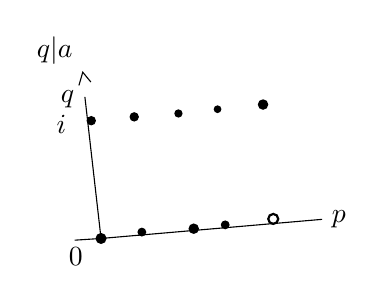
\begin{tikzpicture}[x=.54cm,y=.54cm]
\draw (0,0)--(-.38,3.33);
\draw (-.52,3.60)--(-.43,3.91)--(-.24,3.68);
\node[above left] at (-.44,3.86) {$\unsure{q|a}$};
\draw (-.62,-.04)--(0,0)--(5.2,.45) node[right] {$p$};
\node[below left] at (-.20,.02) {$0$};
\node[left] at (-.59,2.69) {$i$};
\node[left] at (-.40,3.27) {$\deleted{\unsure{q}}$};
\fill (0,0) circle (2pt) (.96,.15) circle (1.6pt) (2.18,.23) circle (1.9pt) (2.92,.32) circle (1.6pt);
\draw[thick] (4.05,.46) circle (1.8pt);
\fill (-.23,2.77) circle (1.7pt) (.78,2.86) circle (1.7pt) (1.82,2.94) circle (1.5pt) (2.74,3.04) circle (1.4pt) (3.81,3.15) circle (1.9pt);
\end{tikzpicture}}

\diagram{\begin{tikzcd}[ampersand replacement=\&]
0\arrow[r] \& H^{\deleted{\unsure{p}}i}(C(U^{*},F))\arrow[r] \& H^{\deleted{\unsure{p}}i}(\mathscr X,F)\arrow[r] \& H^0\bigl[\underbrace{H^{\deleted{\unsure{p}}i}(U^{*},F)}_{\substack{\text{complexe}\\\text{cosimplicial}\\\text{pour }p}}\bigr)\\
\&\&\rotatebox{90}{$\in$}\&\Vert\\
\&\&\xi\&\operatorname{Ker}\bigl(H^i(U,F)\rightrightarrows H^i(U^2,F)\bigr)
\end{tikzcd}}

\unsure{$1$} \unsure{de sorte} Par hypothèse sur $U$, l'image de $\xi$ dans le troisième terme est nulle, donc $\xi$ appartient au premier terme. Mais \inserted{par $(\alpha)$,} le complexe $C(U^\bullet,F)$ est \deleted{\unsure{celui de}} le complexe \uline{trivial} des puissances de $I=\pi_0(U)$, à coeff. \inserted{dans $M$} (car $F=M_{\mathscr X}$). Sa cohomologie

% archive sheet number: 173
\scanpage{174}
\mspage{32}

\inserted{en degrés $>0$} est nulle, donc $\xi=0$, \unsure{qed.|cqfd.}

% slanted
\reversemarginpar\margin{C'est déjà dans SGA4 I 8}\normalmarginpar

\uline{Proposition} 2.15. Soit $X$ un objet de Cat. Conditions équivalentes :

a) $X$ est filtrante, i.e. $X$ est $0$-connexe et $X^{\unsure{o|0}}$ satisfait les conditions \unsure{équiv.} du th. 2.6 ($X^{o\,\wedge}$ est loc. tot. $0$ connexe).

b) \deleted{\unsure{tous les objets foncteurs}} L'objet final de $X^\wedge$ est ind-représentable.

\uline{Dém.} On sait qu'on a

\[
e_{X^\wedge}\simeq\varinjlim_{x\in X}x,\tag*{(2.15.1)}
\]

limite inductive prise dans $X^\wedge$. En effet, cela signifie aussi que pour tout objet $a$ de $X$, on a

\[
\varinjlim_{x\in X}\underbrace{x(a)}_{\operatorname{Hom}_{X}(a,\unsure{X|x})}\xrightarrow{\sim}e
\quad\text{(\unsure{ens. un elt|ens. ensbl} ponctuel)}.
\]

Mais \unsure{considérons} l'\deleted{\unsure{espace}} \inserted{objet} \deleted{étale} $X'={}_{a}\backslash X\deleted{\unsure{_{/a}}}\unsure{\mathbin{-}|\longrightarrow}X$ coétale sur $X$, qui est \inserted{au \unsure{Cat-|cat-}} \unsure{cofibrée|cofibré} sur $X$, on sait que l'on a

\[
\pi_0(X'\deleted{\unsure{_{/x}}})\simeq\varinjlim_{x\in X}\deleted{\unsure{X_x}}\pi_0(X'_x),\quad\text{or}
\]

$X'_x=\operatorname{Hom}(a,x)$, donc on trouve

\[
\varinjlim_{x\in X}\operatorname{Hom}(a,x)=\pi_0({}_{a}\backslash X).=e
\]

car $\,{}_{a}\backslash X$ est $0$-connexe

La formule (2.15.1.) montre que si

% archive sheet number: 174
\scanpage{175}
\mspage{33}

$\unsure{X|\mathscr X}$ est filtrante, $e_{X^\wedge}$ est limite inductive filtrante de foncteurs représentables. On sait d'ailleurs qu'on peut réindexer par \unsure{une|un} catégorie \uline{ordonnée} filtrante (cf SGA4, I, \S\,8.1.6 (c'est dû à P. Deligne ?).

On a prouvé $a\Longrightarrow b$, prouvons $b\Longrightarrow a$. Supposons donc

\[
e_{X^\wedge}=\varinjlim_{i\in I}x_i,
\]

où $I$ est un \inserted{(petit)} ens. ordonné filtrant, et $I\longrightarrow X$ un foncteur. \deleted{Soit \unsure{Prouvons}} Prouvons PS1$'$ \inserted{(forme \unsure{droite|duale})} i-e. pour $a,b$ dans $X$, existe

\diagram{\begin{tikzcd}[ampersand replacement=\&]
a\arrow[r] \& x\\ b\arrow[ur]\&
\end{tikzcd}}

. En effet, \deleted{il ex\unsure{.}} comme \deleted{\unsure{$\varinjlim\operatorname{Hom}(a,x)$}} $\varinjlim_I\operatorname{Hom}(a,x_i)=e$, il s'ensuit que $\operatorname{Hom}(a,x_i)\ne\varnothing$ pour $i$ grand, de $=$ $\operatorname{Hom}(b,x_i)\ne\varnothing$, donc il suffit de prendre

\diagram{\begin{tikzcd}[ampersand replacement=\&]
a\arrow[r] \& x_i\\ b\arrow[ur]\&
\end{tikzcd}}

. Prouvons $\mathrm{PS2}_{\unsure{d|a}}$, i.e. que pour double flèche $a\overset{u}{\underset{v}{\rightrightarrows}}b$, existe $b\unsure{\mathbin{-}|\longrightarrow}x$ qui égalise. Considérons,

\deleted{\unsure{Hom} $i\to j$, $\exists$ \unsure{compatible}, \unsure{$x_i\to x$}}

\diagram{\begin{tikzcd}[ampersand replacement=\&]
\deleted{\xi_i\in\operatorname{Hom}(b,x_i)}\arrow[d]\arrow[r,shift left=.6ex,"{\deleted{u^*}}"]\arrow[r,shift right=.6ex,"{\deleted{v^*}}"']\&\deleted{\operatorname{Hom}(a,x_i)}\arrow[d]\\
\deleted{\lim\operatorname{Hom}(b,x_i)}\arrow[r,"{\deleted{\sim}}"]\&\deleted{\lim\operatorname{Hom}(a,x_i)=e}
\end{tikzcd}}

% archive sheet number: 175
\scanpage{176}
\mspage{34}

Soit $\xi_{i_0}^{\unsure{\xi|\vphantom{\xi}}}$ dans $\operatorname{Hom}(b,x_{i_0})$, ses deux images dans $\operatorname{Hom}(a,x_{i_{\unsure{0|\vphantom{0}}}})$ ne sont pas néc. égales, mais le \unsure{deviennent|sentent} dans la limite inductive, réduite à $e$, donc \deleted{qu'elles sont égales} \inserted{deviennent égales en} composant avec $x_{i_0}\to x_i$, pour $i$ assez grand, donc le composé $b\unsure{\mathbin{-}|\to}x_{i_0}\mathbin{-}x_i$

\[
a\overset{\displaystyle\longrightarrow}{\unsure{\longrightarrow|-}}b\longrightarrow x_{i_0}\mathrel{\unsure{\to|-}}x_i
\]

\deleted{\unsure{il en}} égalise la double flèche.

\uline{Corollaire} 2.16. Soit $W$ un localiseur fondamental satisfaisant l'axiome des limites $\mathrm{Loc}\,(\unsure{d^\circ|*|L^\circ})$. Si $X$ \inserted{dans Cat} est une catégorie filtrante ou cofiltrante, alors $X$ est $W$-asphérique.

Plus généralement et agréablement :

% slanted
\reversemarginpar\margin{cf $\underline{\overline{\mathrm{XII}}}$ \S\ \uline{V} : pour cette notion, que j'ai beaucoup peiné à dégager et à comprendre !}\normalmarginpar

\uline{Corollaire} 2.17. Soit $W$ comme dans 2.16. Alors \deleted{\unsure{toute}} catégorie filtrante \uline{\unsure{totalement} $W$-asphérique}, i-e pour \deleted{tout, foncteur} \unsure{flèche} $f:X\longrightarrow Y$ dans Cat, \deleted{la catégorie \unsure{$f_!(X/Y)$}} l'objet $f_!(e_X)$ de $e_Y$ \deleted{est $W$-asphérique,} (défini aussi comme \deleted{l'espace} $y\longmapsto\pi_0({}_{y}\backslash X)$, et intervenant dans la factorisation canonique de $f$ en \deleted{\unsure{épi}}, en \unsure{p.} étale et \unsure{en|les} \unsure{cofibration|cofibres} \deleted{\unsure{de|des}} \unsure{fibr. à|fes b} \inserted{$0$-connexes})

% archive sheet number: 176
\scanpage{177}
\mspage{35}

est $W$-asphérique. En fait, $Y_{/f_!(e_{X^\wedge})}$ est \inserted{\unsure{elle}} $=$ une catégorie filtrante.

En effet, le foncteur $f_!$ commute aux limites inductives, \deleted{donc} $f_!e_{X^\wedge}$ est limite inductive filtrante des $f_!(x_i)=f(x_i)$. Donc $Y_{/f_!(e_{X^\wedge})}$ est limite inductive filtrante des $Y_{/f(x_i)}$, Donc \deleted{il est} \inserted{c'est} $=$ une catégorie filtrante, a fortiori \deleted{\unsure{elle est}} $W$-asphérique.

Donc \unsure{finalement|facilement}, on trouve des exemples non triviaux de catégories tot. $W$-asphériques, \unsure{i.e. des} exemples dans des catégories sans objet final.

% slanted
\reversemarginpar\margin{déjà dans SGA4 I 8 \rule{0.4pt}{4ex}}\normalmarginpar

\uline{Corollaire} 2.18. Soit $X$ dans \unsure{Cat}, $F$ dans $X^\wedge$. Pour que $F$ soit ind-représentable, il f. et s. que $X_{/F}$ soit filtrante.

En effet, \inserted{par (2.15;)} $X_{/F}$ est filtré ssi l'objet final $F$ de $X_{/F}$ \deleted{est limite inductive} \inserted{provient d'un} \deleted{d'une famille filtrante} ind-objet de $X_{/F}$, mais cela signifie aussi que $F$ est la limite inductive dans $X^\wedge$ d'un ind-objet de $X$, i.e. que $F$ est ind-représentable.

% archive sheet number: 177
\scanpage{178}
\mspage{36}

\uline{Question} Si $X$ dans Cat est tot. $W_\infty$-asphérique, i.e. les $f_!(e_{X^\wedge})$ sont $W_\infty$-asphériques pour tte flèche $f:X\to Y$ de Cat, ou encore pour tte telle flèche, avec les $\,{}_{y}\backslash Y$. $0$-connexes ($y\in\operatorname{Ob}Y$), $Y$ est $W_\infty$-asphérique -- cela implique-t-il que $X$ soit \unsure{($'$)} filtrante ? Ça ne m'étonnerait pas, et $=$ \deleted{\unsure{en}} supposant seulement les $f_!(e_{X^\wedge})$ $1$-connexes$^*$ -- (ils sont $0$-connexes, dès que $X$ l'est). Mais je ne veux pas m'attarder à présent sur cette question\unsure{\ldots}

% slanted
\reversemarginpar\margin{\deleted{\uline{Non}, cf \unsure{plus bas}}}\normalmarginpar

% slanted
\reversemarginpar\margin{Ils le sont toujours \unsure{aussi|ainsi} (cf $\underline{\overline{\mathrm{XII}}}$ plutôt), cf \unsure{\S\,?} \unsure{c'est} \uline{\unsure{2-connexe}} qu'il faut lire \unsure{depuis tjrs|de suite} !}\normalmarginpar

La réponse à la question précédente est négative, comme on voit par la prop.

% slanted
\reversemarginpar\margin{\uuline{Faux} $\longrightarrow$ cf \unsure{déf. 3.3}, p.~45}\normalmarginpar

\uline{Prop.} 2.19. Soit $X$ \deleted{une catégorie} \inserted{de Cat}, telle que $\operatorname{diag}_X:X\to X\times X$ soit cofinale$^*$, i.e. telle que $X^{\unsure{o|0}}$ soit tot. $0$-connexe. Alors $X$ est tot. $\mathbb W_\infty$-asph. (donc aussi tot $W$-asphérique, pour tt \unsure{loc.} fond. \deleted{\unsure{tot}} tel que $W\supset\mathbb W_\infty$).

Soit en effet un foncteur cofinal $f:X\to Y$, il faut prouver que $Y$ est $\mathbb W_\infty$-asph. Or on sait que tot-$0$-connexe implique $\mathbb W_\infty$-asph.$^*$ (cf prop. 2.3 p.~17-18), donc il suffit de voir que $Y^o$ est tot. $0$-conn., i.e. $Y\xrightarrow{\deleted{\unsure{\to}}d_Y}Y\times Y$ cofinal. Or on a le diagramme commutatif

% slanted
\reversemarginpar\margin{C'est \uuline{faux}}\normalmarginpar

\diagram{\begin{tikzcd}[ampersand replacement=\&]
X\arrow[r,"d_X"]\arrow[d,"f"']\&X\times X\arrow[d,"f\times f"]\\
Y\arrow[r,"d_Y"']\&Y\times Y
\end{tikzcd}}

où par hypothèse $f$, donc aussi $f\times f$, et $d_X$ sont cofinaux. Donc $g=(f\times f)\circ\unsure{p_X|d_X}$ est cofinal, et comme $g=d_Yf$ et $f$ est aussi cofinal, on conclut que $d_Y$ l'est, qed.

\uline{Corollaire} $\mathord{\tikz[baseline=0pt,x=1em,y=1em]{\draw (0,0)--(.45,.72)--(.74,0)--cycle; \draw (.13,.025)--(.48,.63);}}^{\deleted{\unsure{o}}}$ \deleted{\unsure{étant}} tot. $0$-conn, $(\mathord{\tikz[baseline=0pt,x=1em,y=1em]{\draw (0,0)--(.45,.72)--(.74,0)--cycle; \draw (.13,.025)--(.48,.63);}})^o$ est \inserted{tot.} $\mathbb W_\infty$-asph. pourtant il n'est pas filtrant.

% slanted
\margin{Question ($X$ \deleted{\unsure{tot.}}$-\mathbb W_\infty$-asph $\Rightarrow X^o$ tot. $0$-connexe ? On dirait \unsure{oui} puisque \unsure{PS$'1$} \unsure{--}}

% archive sheet number: 178
\scanpage{179}
\mspage{36 bis}

\inserted{2.20.} Contr'exemple à la proposition fausse 2.19.

Soit $X$ un\deleted{\unsure{e catég}} objet de Cat, rajoutons lui \deleted{un objet} la catégorie finale $e$ comme fermé, i.e. considérons un objet $X'$ de Cat dans lequel $X$ soit un sous objet ouvert, $e$ le fermé complémentaire :

\diagram{\begin{tikzcd}[ampersand replacement=\&]
X\arrow[r,hook,"i"] \& X' \& e\arrow[l,hook',"j"']
\end{tikzcd}}

On sait (cf $\underline{\overline{\mathrm{XII}}}$) qu'une telle opération est déterminée, à isom. près, par la donnée d'un objet

\[
H\in\operatorname{Ob}X^\wedge,
\]

en posant

\[
H(x)=\operatorname{Hom}_{X'}(x,e),
\]

la catégorie $X_{/e}$ s'identifiant (à isom près) à $X_{/H}$. Elle est donc $0$-connexe ssi l'objet $H$ de $X^\wedge$ est $0$-connexe. Cela signifie aussi que le morphisme $i$ est cocofinal, i.e. que $i^{\unsure{o|0}}:X^o\hookrightarrow X'^{o}$ est cofinal. Supposons maintenant $X$ $\mathbb W_\infty$-asphérique et tot. $0$-connexe \deleted{($W$ étant un loc. fond. satisfaisant $W(\unsure{\mathrm{As}|\lim})$)}, i.e l'actuel Loc(6), cf $\underline{\overline{\unsure{\mathrm{XVI}|\mathrm{XVII}}}}$.) La proposition 2.19 affirme que sous ces conditions, $X'$ (qui \unsure{est} lui aussi tot $0$-connexe) est $=$ $W$-asphérique. Il s'ensuivrait \deleted{que} donc que $i\in\mathbb W_\infty$. Mais par $\underline{\overline{\mathrm{XII}}}$ th. 4 cor. \unsure{4|5} (p.~149) il s'ensuivrait que

% archive sheet number: 179
\scanpage{180}
\mspage{36 ter}

$X_{/e}$ est $\mathbb W_\infty$-asphérique, i.e $H$ $\mathbb W_\infty$-asphérique. Ainsi, si $X$ est tot. $0$-asphérique, tout objet $0$-connexe \unsure{de} $X^\wedge$ serait $\infty$-connexe. Mais c'est manifestement faux, p. ex. si on prend pour $X$ une catégorie-test pour $\mathbb W_\infty$, p. ex. $X=\mathord{\tikz[baseline=0pt,x=1em,y=1em]{\draw (0,0)--(.45,.72)--(.74,0)--cycle; \draw (.13,.025)--(.48,.63);}}$.

Cela me fait soupçonner que la conjecture

\[
X\ \text{\unsure{tot.}}\ \mathbb W_\infty\text{-asphérique}\ \Longrightarrow X\ \text{filtrante}
\]

pourrait être valable.

% archive sheet number: 180
\scanpage{181}
\mspage{37}

3. \uline{Retour sur la cofinalité}.

Il est instructif de relier les questions de cofinalité (pour une flèche $u:I'\mathbin{-}I$ dans $\mathrm{Cat}$) au dérivateur $\mathrm{HOT}_{W^{\deleted{\unsure{*|\infty}}}_0}$, où $W^{\deleted{\unsure{*|\infty}}}_0\subset\mathrm{Fl}\,\mathrm{Cat}$ est le plus grossier des localiseurs dans $\mathrm{Cat}$ satisfaisant l'axiome de connexité $\mathrm{Loc}\,5$,

\unsure{i.e}

\[
W_0=\bigl\{f\in\mathrm{Fl}\,\mathrm{Cat}\ \big|\ \pi_0(f)\ \text{bijectif}\bigr\}\tag*{(3.1.)}
\]

On trouve alors, \unsure{pour} $I$ dans $\mathrm{Cat}$, une équivalence canonique, $2$-fonctorielle en $I$

\[
\mathrm{HOT}_{W_0}(I)\xrightarrow{\approx}I^\wedge\overset{\mathrm{def}}{=}\underline{\mathrm{Hom}}(I,(\mathrm{Ens}))\tag*{(3.2.)}
\]

en d'autres termes on a une équivalence

\[
\mathrm{HOT}_{W_0}\simeq\mathbb D_{(\mathrm{Ens})}\,.\tag*{(3.3.)}
\]

Quand $\mathrm{HOT}_{W_0}(I)$ est défini par localisation à partir de la catégorie $\mathrm{Cat}(I)\overset{\mathrm{def}}{=}\underline{\mathrm{Hom}}(I^o,\mathrm{Cat})$, la flèche 3.2. est celle déduite, par localisation, de la flèche

\[
\begin{aligned}
\pi_0^I:\ \underline{\mathrm{Hom}}(I^o,\mathrm{Cat})&\unsure{\longrightarrow|\mathbin{-}}\underline{\mathrm{Hom}}(I^o,(\mathrm{Ens}))\\
X\deleted{\unsure{_{*}|_{/}}}&\longmapsto\pi_0\circ X
\end{aligned}\tag*{(3.4)}
\]

\deleted{\unsure{$\pi$}}

\[
\pi_0:\mathrm{Cat}\mathbin{-}(\mathrm{Ens})\tag*{\unsure{(3.5)|(2.5)}}
\]

est le foncteur ``composantes connexes''.

Si l'on décrit $\mathrm{HOT}_{W_{\unsure{0|1}}}(I)$ comme localisé de $\mathrm{Cat}_{/I}$, (3.2), est déduite de la flèche

\[
\left\{\begin{aligned}
\mathrm{Cat}_{/I}&\longrightarrow\deleted{\unsure{I^\wedge|I}}\,I^\wedge=\underline{\mathrm{Hom}}(I^o,(\mathrm{Ens}))\\
X&\longmapsto\deleted{\unsure{\xi|X}}\,\pi_0(X/I)=(i\mapsto\pi_0(i\backslash X))\end{aligned}\right.\tag*{(3.6)}
\]

% archive sheet number: 181
